\documentclass[a4paper,twoside,12pt]{scrreprt}
\usepackage{diplomski}

% Ne znam
\pagestyle{headings}

% Podrška za hrvatski
\usepackage[croatian]{babel}
\usepackage[utf8]{inputenc}
\usepackage[T1]{fontenc}

% Veći razmak između paragrafa
\setlength{\parskip}{\bigskipamount}
% Makni indentaciju na početku paragrafa
\setlength{\parindent}{0pt}
% Dodaj kompaktnije liste
\usepackage{paralist}
% Quoting okruženje s manje razmaka
\usepackage{quoting}
\quotingsetup{vskip=0pt}
% Centriranje bez dodatnog razmaka
\newenvironment{nscenter}
 {\par\nopagebreak\centering}
 {\parskip=0pt\par\noindent\ignorespacesafterend}

% Pretvori linkove u hyperlinkove
\usepackage{hyperref}
% Pretvori URLove u hyperlinkove
\usepackage{url}

% Degree symboli
\usepackage{gensymb}
% Specificiranje tipa numeriranja
\usepackage{enumerate}

% Omogući slike
\usepackage{graphicx}
% Omogući popis slika
\usepackage{float}
% Promjeni defaultni folder za slike
\graphicspath{{./images/}}

\title{Računalna obrada teksta}
\author{Janko Marohnić}
\advisor{Prof. dr. sc. Robert Manger}
\date{Travanj, 2015.}

\begin{document}

\frontmatter

\chapter{Uvod}

Kada se informacije premjeste iz fizičkih papira u digitalni format, moguće ih analizirati i pretraživati uporabom računala. Kroz godine su razvijene razne metode i tehnike obrade teksta koje su znatno unaprijedile organizaciju tih digitalnih informacija. U nastavku ćemo jednu sadržajnu cjelinu informacija (knjiga, članak i sl) koja može imati više polja (naslov, autor itd) zvati \textit{dokument}.

Postoje razni korisni rezultati koji se mogu postići današnjim metodama obrade teksta. Primjerice, moguće je grupirati nepovezanu kolekciju dokumenata po sličnosti (eng. \textit{clustering}), te korisniku koji čita jedan dokument ponuditi druge, sadržajno \textit{povezane} dokumente (eng. \textit{more like this}). Također, moguće je iz dokumenata izvaditi najbitnije pojmove, i tako saznati glavnu temu dokumenta. I naravno, moguće je pretraživati sve dokumente po nekom upitu. Od svih navedenih značajki, pretraživanje je jedina značajka koja neophodna za upravljanje digitalnim informacijama, te će ono biti tema ovog rada.

Bez mogućnosti kvalitetnog pretraživanja korisnik najčešće neće moći pronaći željeni dokument, jer je u većini aplikacijama broj dokumenata jednostavno prevelik. A ako korisnik ne može pronaći neki dokument, on efektivno ne postoji. To nije veliki problem ako se radi o aplikaciji kao što su web novine. Međutim, za web dućane korisnikova nemogućnost da pronađe određeni artikl znači da korisnik taj artikl ne može niti kupiti, a za web tražilice (npr. \textit{Google}) korisnikova nemogućnost da pronađe određenu web stranicu znači da joj on ne može pristupiti. Dakle, većini aplikacija mogućnost kvalitetnog pretraživanja nije samo luksuz, već je značajka koja je neophodna za njihovu egzistenciju.

Budući da se informacije obično sastoje od velikih količina teksta, u ovom radu ćemo se orijentirati na tzv \textit{pretraživanje punog teskta} (eng. \textit{full-text search}). Za kvalitetno pretraživanje punog teksta, nažalost, općenito nisu dovoljne klasične relacijske baze podataka (MySQL, PostgreSQL, Oracle). Dok su takve baze podataka vrlo efikasne za pretraživanje po diskretnim vrijednostima polja, one obično manjkaju sposobnosti kada treba odrediti koliko neki dokument ispunjava neki tekstualnom upitu. Točnije ne znaju efikasno odrediti koja polja dokumenta ispunjavaju koji dio upita (koji se sastoji od običnog niza znakova), i tako odrediti koliko je taj dokument relevantan upitu. Iako klasične baze podataka podržavaju regularne izraze, kvalitetno pretraživanje punog teksta zahtijeva više od jednostavnog uspoređivanja znakova. Takva tražilica treba moći unaprijed obraditi tekst da maksimalno ubrza vrijeme izvršavanja upita. Ona treba moći zanemariti eventualne zatipke (eng. \textit{typo}) korisnika, i ne ograničavati se na specifične padeže i veličine slova. Konačno, ona treba vratiti rezultate rangirane po relevantnosti. U sljedećem poglavlju obradit ćemo glavne značajke koje tražilice punog teskta trebaju imati.

Aplikacija, da može pružiti svojim korisnicima mogućnost pretraživanja, može izabrati ili sama implementirati svoju tražilicu, ili koristiti jedan od već postojećih softvera. Budući da je danas kvaliteta javno dostupnih tražilica dosegla razinu gdje je dovoljna za vodeće svjetske aplikacije, nema razloga ne odlučiti se za potonju opciju. U radu ću spomenuti i obraditi sve vodeće softvere za pretraživanje, ali isključivo one otvorenog koda (eng. \textit{open source}). Naime, tražilice otvorenog koda su se pokazale da izvrsno funkcioniraju i za svjetski popularne aplikacije (npr. Wikipedia), pa obično nema razloga za korištenje komercijalnih.

Za praktični dio rada izradit ću vlastitu web aplikaciju u kojoj ću implementirati pretraživanje određene količine dokumenata koristeći svaku od vodećih tražilica. Cilj praktičnog dijela je usporedba vodećih tražilica u aspektima brzine pretraživanja i jednostavnosti korištenja.

\chapter{Pretraživanje}

U ovom poglavlju obradit ćemo sve glavne elemente koje čine tražilicu punog teksta. Proces pretraživanja može se opisati u četiri dijela:

\begin{compactenum}
  \item \textbf{Indeksiranje} – Datoteke i baze podataka obrađuju se i pripremaju za pretraživanje
  \item \textbf{Upit} – Korisnik upisuje ključne riječi kroz neku vrstu korisničkog sučelja, i tražilica pronalazi sve dokumente koji ispunjavaju upit
  \item \textbf{Rangiranje} – Tražilica rangira pronađene dokumente s obzirom koliko dobro ispunjavaju upit
  \item \textbf{Prikaz rezultata} – Konačni rezultati se prikazuju u korisničkom sučelju.
\end{compactenum}

\section{Indeksiranje}
\label{indexing}

\textit{Indeksiranje} je proces analize unešenih podataka, čiji se rezultati formiraju u sadržaj (\textit{indeks}) koji se može spremiti na disk, i kasnije se koristiti za brže pretraživanje. U tradicionalnim relacijskim bazama indeksiranje podataka je opcionalno; preporuča se za veće količine podataka radi brzine, ali može se izostaviti kada je podataka dovoljno malo da ne bi bilo znatne razlike u brzini. Tražilice punog teksta, s druge strane, zahtijevaju da se svi podaci (dokumenti) indeksiraju, te to rade automatski pri unosu. Naime, značajke pretraživanja punog teksta su puno kompleksnije od standardnog pretraživanja, te ih ne bi bilo moguće realizirati u razumnoj brzini kada bi se dokumenti analizirali tek za vrijeme upita.

Indeksiranje za pretraživanje punog teksta može se podijeliti u tri dijela:

\begin{compactenum}
  \item Preprocesiranje
  \item Analiza
  \item Spremanje
\end{compactenum}

\subsection{Preprocesiranje}

Prije samog obrađivanja, potrebno je sve dokumente svesti na jednu zajedničku tekstualnu reprezentaciju. Pretpostavimo da radimo aplikaciju koja omogućuje pohranjivanje digitalnih prezentacija, koje se učitavaju u PDF formatu, i koje se onda mogu gledati online\footnote{Jedna takva aplikacija je \url{http://speakerdeck.com}.}. Htjeli bismo omogućiti da korisnici mogu pretraživati bazu svih prezentacija po ključnim riječima. Problem je što je PDF tzv \textit{binarni} format, pa nije moguće samo pretraživati sadržaj datoteke. Stoga je potrebno danu PDF datoteku najprije svesti na neki format koje je pogodan za pretraživanje. Taj proces pretvaranja više vrsta datoteka u jednu zajedničku tekstualnu reprezentaciju zove se \textit{preprocesiranje}\footnote{\cite{taming} str. 32}.

Neki od češćih formata datoteki mogu se vidjeti na slici \ref{formats}.

{\renewcommand{\arraystretch}{1.2}
\begin{figure}[H]
  \centering
  \begin{tabular}{|l|l|}
    \hline
    \textbf{Format}                            & \textbf{Esktenzija} \\
    \hline
    Tekst                                      & .txt                \\
    \hline
    Microsoft Office (Word, PowerPoint, Excel) & .doc,.ppt,.xls      \\
    \hline
    Adobe Portable Document Format (PDF)       & .pdf                \\
    \hline
    Rich Text Format (RTF)                     & .rtf                \\
    \hline
    HTML                                       & .html               \\
    \hline
    E-mail                                     & N/A                 \\
    \hline
    Baze podataka                              & N/A                 \\
    \hline
  \end{tabular}
  \caption{Česti formati koji sadrže tekst}
  \label{formats}
\end{figure}
}

Jedan popularan softver otvorenog koda za izdvajanje teksta iz različitih tipova datoteki je Apache Tika\footnote{\url{http://tika.apache.org}}.

\subsection{Analiza}

Nakon što smo sve dokumente sveli na zajednički tekstualni format, moguće je obraditi dokumente na način koji će omogućiti tražilici da ima više značajki, a istovremeno ubrzati samo vrijeme izvršavanja upita.

\subsubsection{Tokenizacija}

Pretraživanje dokumenata svodi se na ispitivanje u kojim se dokumentima pojavljuju ključne riječi unešene u polje za pretraživanje. Svaki dokument se stoga rastavlja na ``riječi'', tzv \textit{tokene}, tako da se onda pretraživanje dokumenata može ugrubo svesti na traženje ključnih riječi u listi tokena.

Međutim, sama tokenizacija nije tako trivijalan zadatak. Pretpostavimo da trebamo tokenizirati sljedeći tekst:

\begin{quoting}
  \textit{Sve današnje skijaške discipline nastale su 1900-1950. godine.}
\end{quoting}

Budući da su riječi odvojene razmacima, promotrimo (naivni) tokenizator \textit{A} koji rastavlja tokene po razmacima:

\begin{nscenter}
  \begin{tabular}{|c|c|c|c|c|c|c|c|}
    Sve & današnje & skijaške & discipline & nastale & su & 1900-1950. & godine.
  \end{tabular}
\end{nscenter}

Dok ovaj pristup funkcionira u nekim slučajevima, primijetimo da se kod našeg teksta na zadnji token nalijepila točka, što ne želimo. Promotrimo sada tokenizator \textit{B} koji odstranjuje interpunkcijske znakove:

\begin{nscenter}
  \begin{tabular}{|c|c|c|c|c|c|c|c|}
    Sve & današnje & skijaške & discipline & nastale & su & 1900-1950 & godine
  \end{tabular}
\end{nscenter}

Dok ovaj tokenizator riješava problem lijepljenja interpunkcijskih znakova za tokene, činjenica da su odstranjeni svi interpunkcijski znakovi stvara novi problem. Pretpostavimo da korisnik pretražuje sve dokumente gdje se pojavljuje fraza ``pobjednik Ivica Kostelić'', i naiđe na sljedeći tekst:

\begin{quoting}
  \textit{Prvo mjesto svjetskog skijaškog kupa odnosi novi pobjednik. Ivica Kostelić, nažalost, osvojio je 25. mjesto u prvoj vožnji i nosi porazno zadnje mjesto.}
\end{quoting}

Ukoliko gledamo strogo koji tokeni se pojavljuju zajedno, fraza ``pobjednik Ivica Kostelić'' bi bila pronađena u ovom tesktu. Ali mi znamo da to ne bi trebalo biti tako, zbog točke nakon ``pobjednik''. Promotrimo zato tokenizator \textit{C} koji odvaja tokene po vrsti znaka: slovo, broj, interpunkcija itd:

\begin{nscenter}
  \begin{tabular}{|c|c|c|c|c|c|c|c|c|c|c|c|}
    Sve & današnje & skijaške & discipline & nastale & su & 1900 & - & 1950 & . & godine & .
  \end{tabular}
\end{nscenter}

Ovdje sve izgleda dobro, riječi su pravilno odvojene, i očuvani su interpunkcijski znakovi. Ovaj pristup također sadrži dodatnu značajku da sada korisnik može upisati ključnu riječ ``1900'' u polje za pretraživanje, i pretraga će pronaći ovaj tekst.

\subsubsection{Normalizacija veličine slova}

U većini aplikacija korisnicima nije važno da dokumenti koje pokušavaju naći sadrže unešene ključne riječi točno jednake veličine. Na primjer, za ključnu riječ ``jabuka'' bi u većini slučajeva imalo smisla da rezultat pretraživanja također uključuje i dokumente koji sadrže riječ ``Jabuka''. Štoviše, kada bi se veličina slova uzimala u obzir, ako bi korisnik htio naći sve dokumente koji sadrže riječ ``jabuka'' bilo na početku ili na kraju rečenice, morao bi proširiti upit na ``jabuka Jabuka''.

Zato se najčešće svim tokenima po konvenciji\footnote{Nije bitno koje su veličine slova, važno je samo da su sva iste veličine} velika slova pretvaraju u mala, čime se efektivno normalizira veličina slova.

\subsubsection{Eliminacija stop-riječi}

\textit{Stop}-riječi su česte riječi poput ``i'', ``ako'' i ``onda''\footnote{U hrvatskom jeziku možemo sve veznike i prijedloge smatrati stop-riječima} koje najčešće nemaju vrijednost za aplikaciju. Na primjer, ako korisnik unese upit ``jabuke i kruške'', a ne postoji niti jedan dokument u bazi podataka koji sadrži riječ ``kruška'' ili ``jabuka'', najčešće ne bi imalo smisla da tražilica onda vrati sve dokumente koji sadrže riječ ``i''.

Iz tog razloga se stop-riječi često izbacuju iz liste tokena. To rezultira i bržim pretraživanjem, jer sada tražilica ima manji broj tokena koje mora pretraživati. Da tražilica može detektirati stop-riječi, potreban joj je digitalni rječnik\footnote{Za najraširenije jezike postoje besplatni online rječnici na \url{http://snowball.tartarus.org}}.

\subsubsection{Normalizacija dijakritičkih znakova}

Hrvatski jezik ima 5 dijakritičkih znakova: \textit{ć}, \textit{č}, \textit{ž}, \textit{š} i \textit{đ}. Međutim, postoje osobe koje ili ne koriste hrvatsku tipkovnicu, ili su stranci koji nemaju puno iskustva u hrvatskom jeziku te možda ne znaju pravilno koristiti dijakritičke znakove. Iz tog razloga se često svi dijakritički znakovi u tokenima zamjenjuju sa njihovim pojednostavljenim verzijama:

\begin{nscenter}
  \begin{tabular}{ccccc}
    ć            & č            & ž            & š            & đ            \\
    $\downarrow$ & $\downarrow$ & $\downarrow$ & $\downarrow$ & $\downarrow$ \\
    c            & c            & z            & s            & d            \\
  \end{tabular}
\end{nscenter}

S tom promjenom korisnici mogu koristiti pojednostavljene verzije riječi u svom upitu, i originalne riječi će još uvijek biti pronađene.

\subsubsection{Korjenovanje}

Pretpostavimo da korisnik želi naći sve dokumente vezane uz banke. Budući da ne zna u kojem obliku i padežu se pojavljuje ta riječ, korisnik bi morao upisivati u tražilicu ``banka banke banci ... banke bankama ... bankarstvo bankarstva ...''. Ovakvo korisničko iskustvo očito nije prihvatljivo; korisnik bi trebao samo upisati riječ ``banka'', i time pretražiti sve varijacije te riječi.

\textit{Korjenovanje} (eng. \textit{stemming}) je proces reduciranja riječi na njen korijen, ili jednostavniji oblik koji sam po sebi ne mora biti riječ\footnote{\cite{taming} str. 25}. Ono omogućuje korisniku da upiše jednu riječ, i dobije natrag sve dokumente koji sadrže bilo koju varijaciju te riječi. Kao i za stop-riječi, za korjenovanje je također potreban digitalni riječnik.

Postoje razni stupnjevi korjenovanja; neki su agresivniji, reducirajući riječi na najmanji mogući korijen, dok su drugi blaži, preferirajući samo osnovnije promjene kao odstranjivanje nastavaka broja i padeža. Svaka aplikacija odabire svoj stupanj korjenovanja, ovisno o željenom omjeru kvalitete i kvantitete. Agresivnije korjenovanje uglavnom vode ka više rezultata ali manjoj kvaliteti, dok blaže korjenovanje može očuvati razinu kvalitete ali uz rizik da neće biti vraćeni neki korisni rezultati. Korjenovanje može uzrokovati probleme gdje se riječi s drukčijim značenjem reduciraju na isti korijen, ili riječi koje su povezane ne reduciraju na isti korijen\footnote{\cite{taming} str. 26}.

Aplikacije mogu najprije početi sa blažim korjenovanjem, pa ga napraviti agresivnijim ukoliko se primjeti da je često vraćeno premalo rezultata. Kao i za eliminaciju stop-riječi, za korjenovanje je također potreban digitalni rječnik.

\subsection{Spremanje}

Nakon što se svi dokumenti tokeniziraju, i ti tokeni normaliziraju obradama navedenim u prethodnoj sekciji, novonastali \textit{termi} (normalizirani tokeni) spremaju se na disk. Konkretno, spremaju se u strukturu zvanu \textit{invertirani indeks} (slika \ref{inverted_index}), koja je optimizirana za brzo pronalaženje dokumenata koji sadrže određen term. Budući da lista termova ne odgovara u potpunosti listi riječi u odgovarajućem dokumentu (jer su odstranjene stop-riječi), u inveritrani indeks se još sprema i pozicija svakog terma unutar dokumenta, zato da bi se omogućile značajke kao pretraživanje po frazama.

\begin{figure}[H]
  \centering
  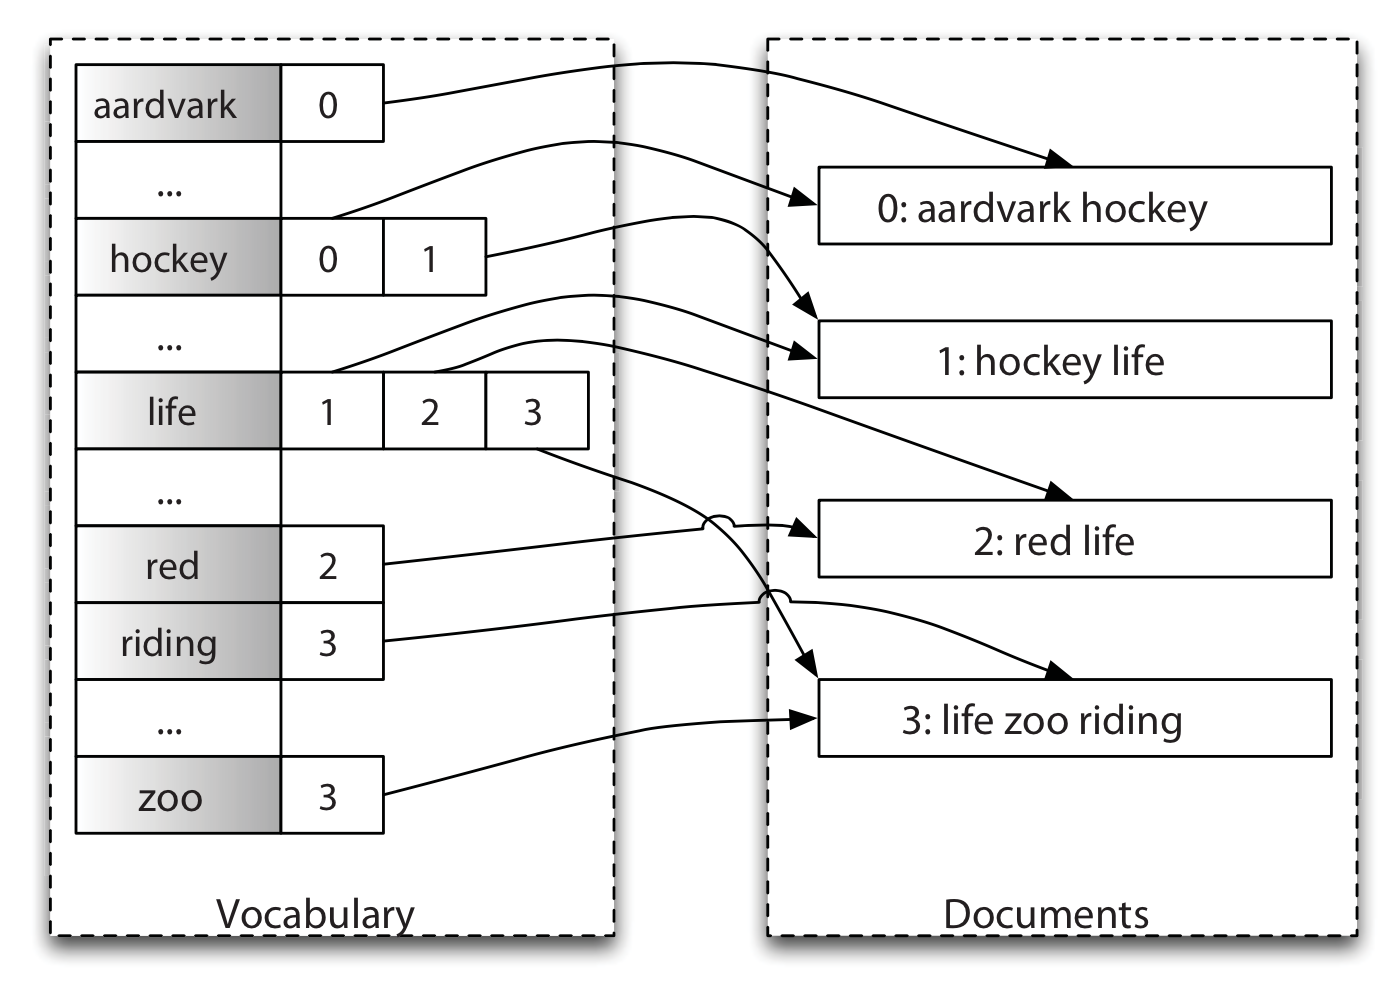
\includegraphics[width=300pt]{inverted_index}
  \caption{Invertirani indeks}
  \label{inverted_index}
\end{figure}

Uz pohranjivanje veza između termova i dokumenata, indeksiranje često uključuje i izračunavanje i spremanje informacija o važnosti termova u odnosu na ostale termove u dokumentu, što je detaljnije objašnjeno u \ref{tfidf}. Ta informacija igra veliku ulogu u omogućavanju tražilice da rangira dokumente po relevantnosti.

\section{Upit}

Nakon indeksiranja tražilica je spremna za upit. Da bi napravio upit, korisnik komunicira kroz neku vrstu korisničkog sučelja, koje prima jedan (``jednostavno pretraživanje'') ili više (``napredno pretraživanje'') upita i vraća odgovarajuću listu dokumenata.

Prije nego tražilica počne pretraživati indeks, sam tekst upita obično prolazi isti postupak obrade kao i dokumenti kada se indeksiraju. Primjerice, ako su tokeni korjenovani u indeksu, onda bi i tokeni iz upita također trebali biti korjenovani. U sljedećim sekcijama ćemo navesti dodatne obrade koje tražilica izvršava na samom upitu.

\subsection{Ključne riječi}

Najosnovniji oblik upita je jednostavno nizanje ključnih riječi odvojenih razmakom (slika \ref{keywords}). Tražilice su obično konfigurirane tako da rezultat takvog upita vrati isključivo dokumente u kojem se nalaze \textit{sve} ključne riječi, da rezultati budu što kvalitetniji. Međutim, ukoliko sama baza aplikacije sadržava vrlo mali broj dokumenata, korisnije je žrtvovati dio kvalitete za kvantitetu, i vratiti sve dokumente koji sadržavaju \textit{bilo koju} od unesenih ključnih riječi.

\begin{figure}[H]
  \centering
  
\includegraphics[width=300pt]{keywords}
  \caption{Primjer upisa ključnih riječi}
  \label{keywords}
\end{figure}

\subsubsection{Dodavanje sinonima}

Kada korisnik upiše ključnu riječ ``pećina'' u polje za pretraživanje, on bi najčešće htio u rezultatima dobiti i dokumente koji sadrže riječ ``špilja''. Iz tog razloga se često upit proširuje sa sinonimima svake riječi. Na primjer, koristeći booleove operatore, upit ``mračna pećina'' bi se mogao proširiti na ``mračna pećina OR špilja''.

Proširivanje sinonimima se vrši na upitu, a ne na indeksu, jer bi se inače indeks znatno povećao (za \textit{svaku} riječ se dodaju \textit{svi} sinonimi), indeksiranje bi općenito dulje trajalo, i indeks bi trebalo obnoviti svaki put kada se list sinonima ažurira.

\subsubsection{Ispravljanje zatipaka}

Pri unosu upita, često se mogu pojaviti zatipci (eng. \textit{typographical error}); bilo zato što korisnik ne zna kako se neka riječ piše (npr. ako piše na engleskom), ili je korisnik jednostavno pritisnuo krivu tipku na tastaturi, i nije to primjetio. Štoviše, zatipci se mogu pojaviti i u tekstu koji se pretražuje.

Zato je uobičajeno da tražilica tolerira određeni stupanj ``greške'' u unosu. Ukoliko tražilica ne pronađe danu riječ u indeksu, ona pokuša pronaći dokumente sa riječima koje su ``slične'' riječi iz upita. Neke tražilice čak idu dalje i u slučaju velike sigurnosti ponude korisniku ispravljenu riječ.

Spomenuli smo pojam međusobne ``sličnosti'' riječi, ali nismo definirali kako se to izračunava. Ovdje je opet od velike pomoći promatranje \textit{n}-grama. Ranije smo radili s \textit{n}-gramima na razini riječi, ali ovaj puta promatramo \textit{n}-grame na razini slova. Najbolja mjera za sličnost dviju riječi je broj njihovih zajedničkih \textit{n}-grama\footnote{\cite{taming} str. 99}, konkretnije trigrama\footnote{\url{http://www.postgresql.org/docs/9.4/static/pgtrgm.html}}.


\subsection{Fraze}

Pretpostavimo da radimo aplikaciju koja omogućuje korisnicima da gledaju riječi pjesama. Pretpostavimo sada da korisnik želi iskoristiti tu aplikaciju da pronađe naziv i autora pjesme na temelju fraza koje je zapamtio iz slušanja te pjesme. Ako korisnik upiše te fraze iz pjesme kao običan niz ključnih riječi, postoji vjerojatnost da će rezultati uključivati i druge pjesme koje sadrže te ključne riječi, i možda pjesma koju korisnik traži neće biti na prvom mjestu. S druge strane, kada bi korisnik mogao reći tražilici da se određeni nizovi riječi iz upita nalaze u dokumentima točno tim redoslijedom, broj vraćenih pjesama se može znatno smanjiti (jer je puno manja vjerojatnost da dvije pjesme dijele čitavu frazu nego par individualnih riječi), i puno je vjerojatnije da će tražena pjesma biti prvi rezultat.

Niz ključnih riječi može se označiti kao fraza tako da se omeđi dvostrukim navodnicima (slika \ref{phrases}). Tražilica pretražuje dokumente za frazu pomoću tzv \textit{n}-grama\footnote{\textit{n}-gram je bilo koji \textit{n}-člani podniz uzastopnih elemenata nekog niza.}. Radi brzine se najprije s manjim \textit{n}-gramima odredi na kojim mjestima je najvjerojatnije da se fraza nalazi, i zatim se ispituju zabilježena mjesta\footnote{\cite{taming} str. 31}.

\begin{figure}[H]
  \centering
  
\includegraphics[width=300pt]{phrases}
  \caption{Primjer upisa fraza}
  \label{phrases}
\end{figure}

\subsection{Booleovi operatori}

Ranije smo spomenuli da za upit ključnim riječima većina tražilica vraća isključivo dokumente koji sadrže \textit{sve} unešene ključne riječi. Međutim, ako primjerice korisnik koristi online dućan mobilnih telefona, i želi pretražiti sve modele Samsunga i iPhonea, tražilica bi trebala omogućiti korisniku da potraži sve dokumente koji sadrže riječ ``iphone'' \textit{ili} ``samsung''.

Zato tražilice obično omogućuju da se između ključnih riječi stave tzv \textit{Booleovi operatori} (slika \ref{boolean}). Operator \textbf{AND} znači da desna i lijeva ključna riječ moraju \textit{obje} biti sadržane u dokumentu, operator \textbf{OR} znači da dokument mora sadržavati \textit{barem jednu} od omeđujućih ključnih riječi, dok operator \textbf{NOT} znači da dokument \textit{ne smije} sadržavati ključnu riječ koja slijedi. Moguće je i korištenje zagrada za gradnju kompleksnijih booleovih izraza.

\begin{figure}[H]
  \centering
  
\includegraphics[width=300pt]{boolean}
  \caption{Primjer booleovih operatora}
  \label{boolean}
\end{figure}

\subsection{Zamjenski znakovi i regularni izrazi}

Naprednijim korisnicima trebalo bi omogućiti maksimalnu preciznost pretraživanja. U tu svrhu može se omogućiti upotreba zamjenskih znakova \textit{?}, koji reprezentira 1 proizvoljan znak, i \textit{*}, koji reprezentira bilo koji broj (uključujući i 0) proizvoljnih znakova (slika \ref{wildcards}). Tako će \textit{bank?} pronaći riječi ``banka'', ``banke'', ``banki'' itd, dok će \textit{bank*} pronaći i riječi kao ``bankama'' i ``bankarstvo''.

\begin{figure}[H]
  \centering
  
\includegraphics[width=300pt]{wildcards}
  \caption{Primjer zamjenskih znakova}
  \label{wildcards}
\end{figure}

Dok su ova 2 zamjenska znakova daju kontrolu dovoljnu u većini slučajeva, postoje neki (rijetki) slučajevi u kojima je potrebna veća preciznost (npr. pretraživanje programskog kôda). Zato neke tražilice u upitu omogućuju i korištenje regularnih izraza\footnote{\url{http://en.wikipedia.org/wiki/Regular_expression}}.

\subsection{Specificiranje polja}

Pretpostavimo da korisnik želi kupiti čvrsti disk, ali ne zna točno koji želi. Korisnik otvori \url{www.nabava.net}, i uđe u kategoriju ``Računala > Pohrana podataka > Čvrsti diskovi'' (slika \ref{nabava1}).

\begin{figure}[H]
  \centering
  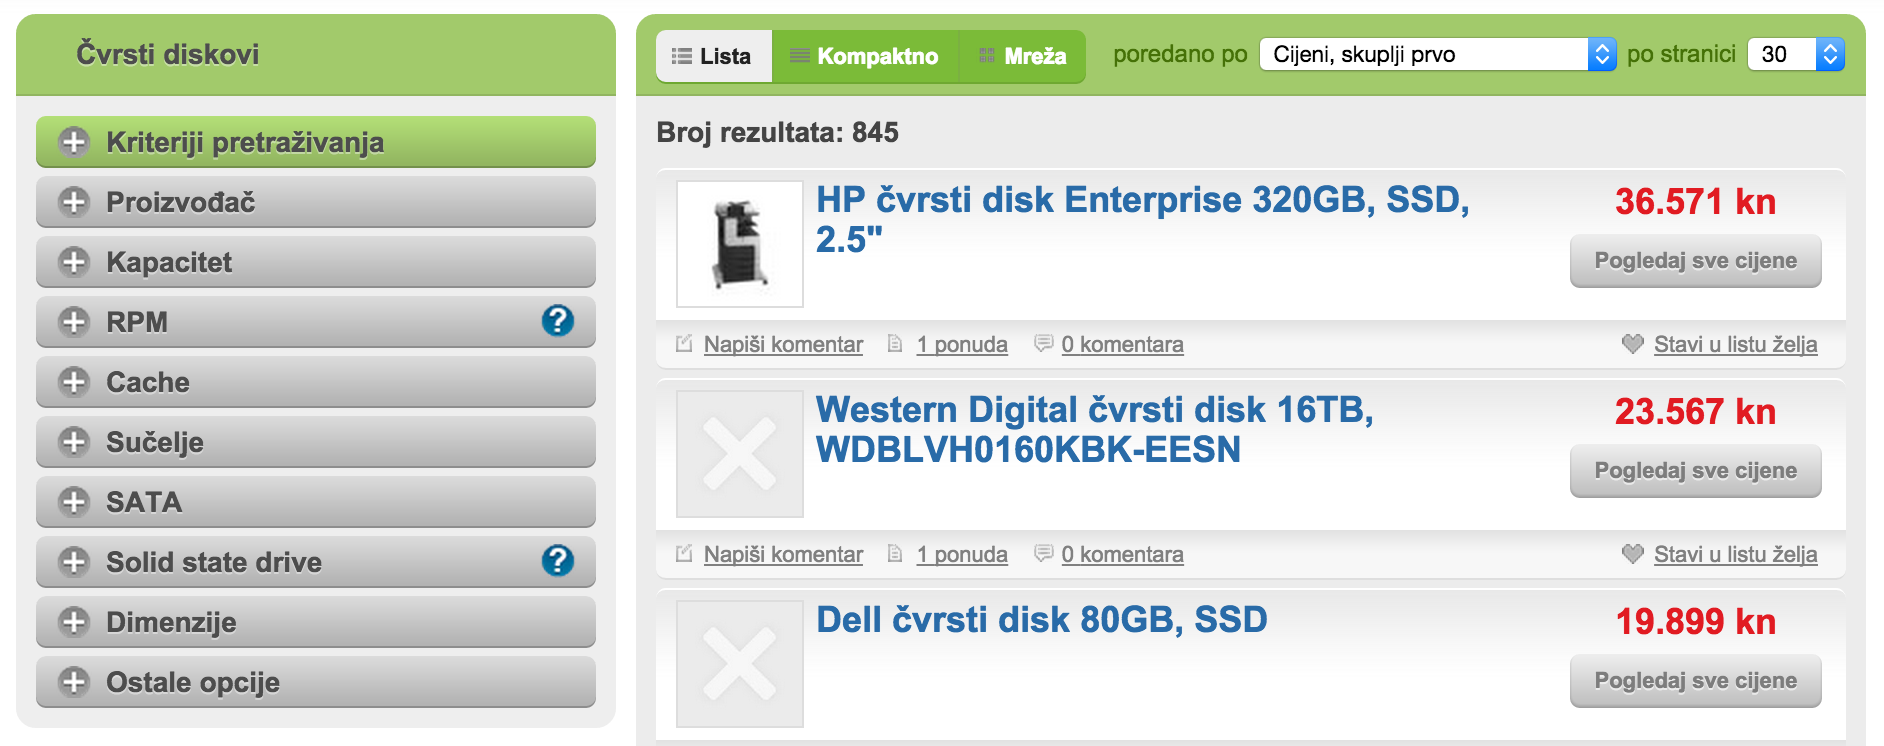
\includegraphics[width=\textwidth]{nabava1}
  \caption{Kategorija ``Čvrsti diskovi'' na \url{www.nabava.net}}
  \label{nabava1}
\end{figure}

Korisnik zatim počne razmišljati koji točno čvrsti disk želi. Prvo, odluči da želi kupiti disk od tvrtke HP, i u lijevom izborniku označi da želi da mu se prikažu svi čvrsti diskovi od te kompanije (slika \ref{nabava2}).

\begin{figure}[H]
  \centering
  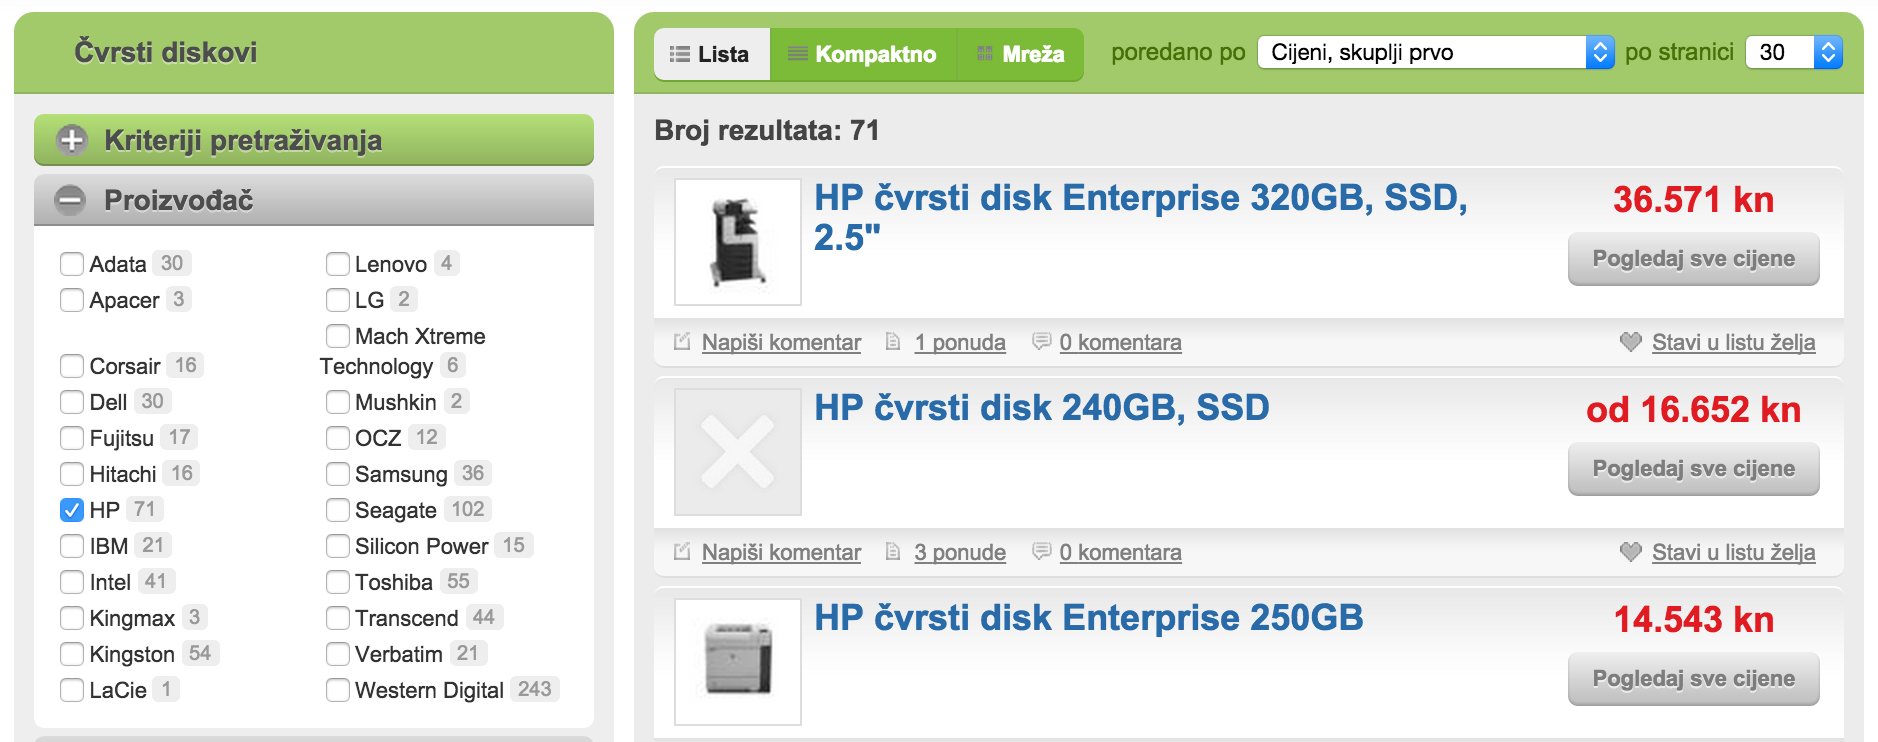
\includegraphics[width=\textwidth]{nabava2}
  \caption{Filtriranje kompanije na \url{www.nabava.net}}
  \label{nabava2}
\end{figure}

Budući da korisnik želi na taj disk uglavnom spremati filmove, odluči da mu treba disk s većim kapacitetom, te u lijevom izborniku označi kapacitet ``512GB - 2TB'' (slika \ref{nabava3}).

\begin{figure}[H]
  \centering
  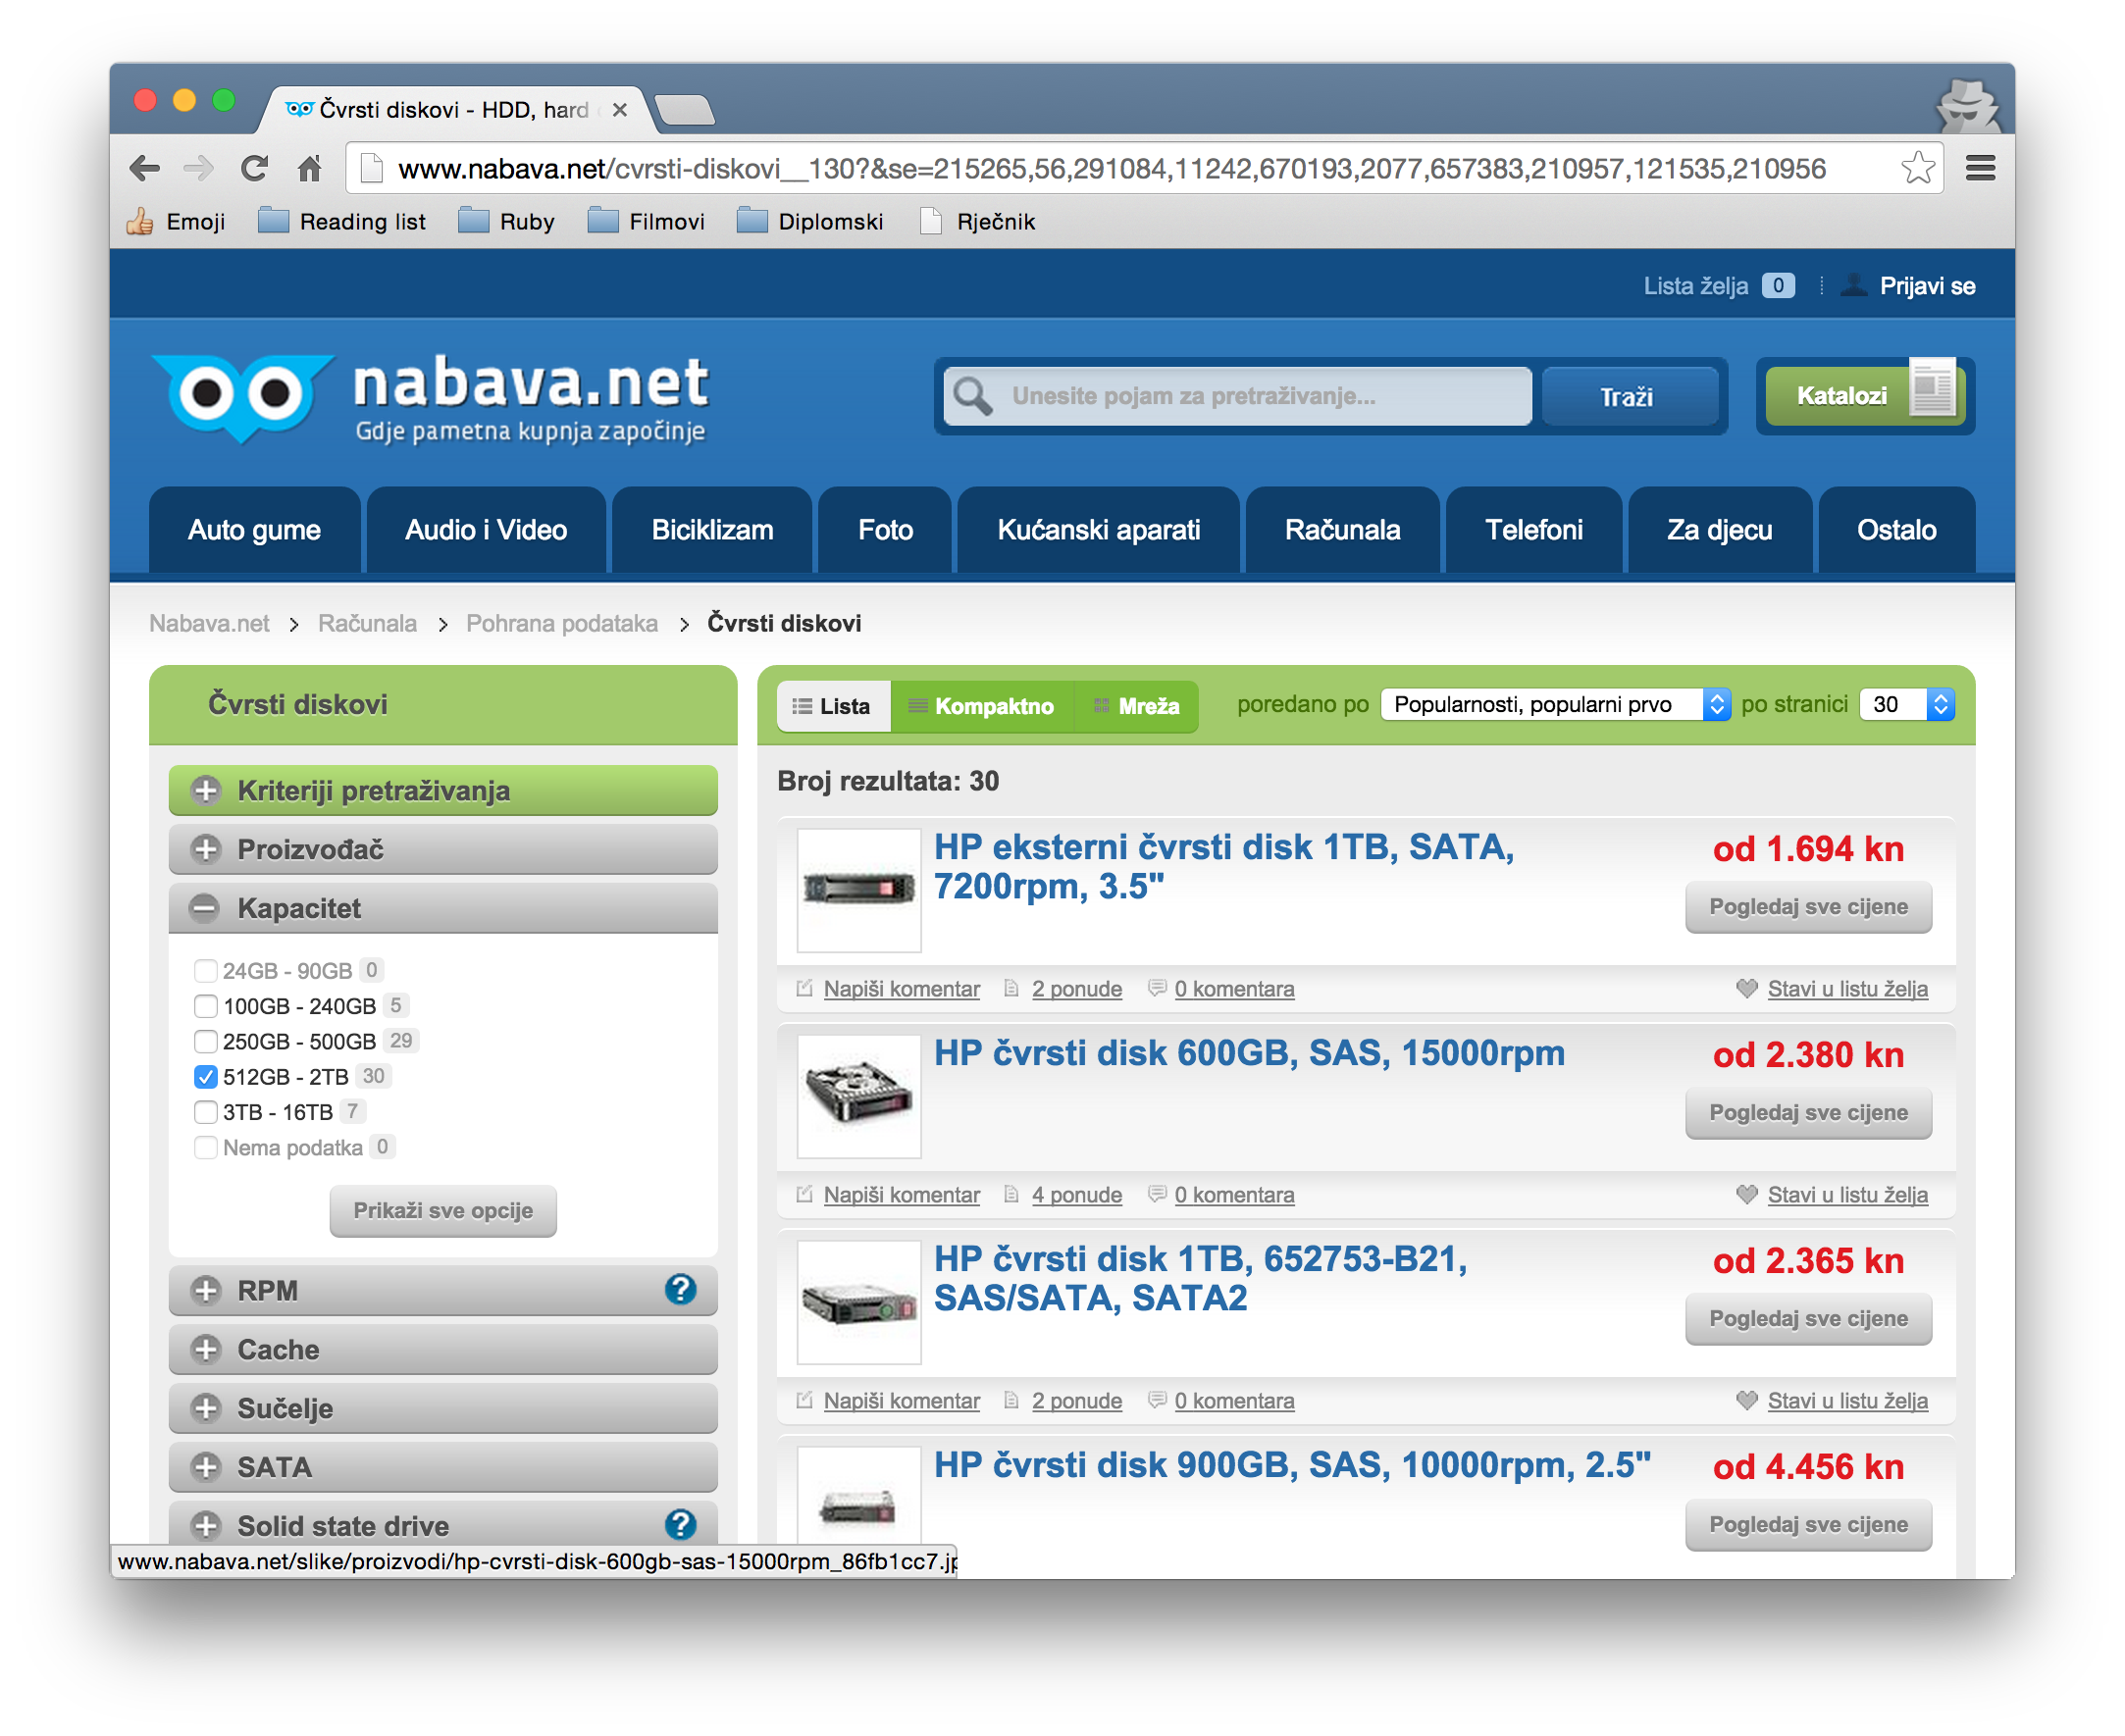
\includegraphics[width=\textwidth]{nabava3}
  \caption{Filtriranje kapaciteta diska na \url{www.nabava.net}}
  \label{nabava3}
\end{figure}

I uz odgovarajuće sortiranje korisnik pronađe željeni disk. Da korisnik nije imao lijevi izbornik koji mu je pomogao filtrirati proizvode po određenim kategorijama, teško bi mogao naći željeni čvrsti disk, jer u ovim slučajevima jedno tekstualno polje za pretraživanje nije dovoljno.

Zato tražilice omogućuju i upite koji će pretraživati specifična polja dokumenata. Gornji primjer je slučaj kada su moguće vrijednosti polja već predefinirane korisniku. Generalno, postoje dvije vrste upita po poljima. Jedna vrsta je upisivanje specifične vrijednosti polja, što je pogodno za tekstualna polja kao što su ``autor'' i ``kategorija''. Druga vrsta je specificiranje nekog intervala vrijednosti, što je pogodno za numerička i vremenska polja kao što su ``cijena'' i ``datum rođenja''.


\subsection{Automatsko nadopunjavanje}

Dok korisnik upisuje znakove u polje za upit, aplikacije često otvaraju listu sugestija iz dokumenata koji se nalaze u indeksu, na temelju znakova koje je korisnik trenutno upisao (slika \ref{typeahead}). (Najčešće se taj niz znakova uzima kao prefix.) To poboljšava korisničko iskustvo na više načina. Prvo, korisniku može skratiti količinu tipkanja tako da korisnik izabere sugestiju umjesto da završi tipkati. Drugo, ako korisnik dobije listu sugestija, onda zna da do sada nije napravio prevelike zatipke. Treće, automatska povratna informacija o korisnikovim upisanim znakovima vodi korisnika da napravi upit koji će sigurno vratiti rezultate.

\begin{figure}[H]
  \centering
  
\includegraphics[width=300pt]{typeahead}
  \caption{Primjer automatskog nadopunjavanja na \url{www.google.com}}
  \label{typeahead}
\end{figure}

Lista sugestija se najčešće dobavlja korištenjem \textit{n}-grama, na sličan način kao kod ispravljanja zatipaka. Najprije se dobavljaju riječi koje sadrže barem jedan zajednički \textit{n}-gram s upitom, a zatim se ta lista rangira po broju zajedničkih \textit{n}-grama\footnote{\cite{taming} str. 100}.

\section{Rangiranje}

Kada tražilica pretražuje sve dokumente koji ispunjavaju dani upit, potrebno je odrediti koliko je neki dokument ``relevantan'' upitu. Iako je tražilicama obično moguće proslijediti opciju sortiranja rezultata po nekom kriteriju (npr. alfabetično ili po cijeni), odsustvo te opcije podrazumijeva da tražilica vraća rezultate sortirane po ``relevantnosti''.

\subsection{Model vektorskog polja}

Da bismo rangirali dokumente, potrebno je definirati mjeru ``relevantnosti'' upitu. Najprije je potrebno postaviti model u kojem ćemo definirati tu mjeru. Postoji mnogo različitih modela, a mi ćemo promatrati najpopularniji – model vektorskog polja.

Ideja modela vektorskog polja je promatranje dokumenata kao vektore u \textit{n}-dimenzionalnom vektorskom prostoru. Vektorski prostor je definiran tako da svaka dimenzija odgovara jednom tokenu iz skupa svih jedinstvenih tokena iz svih dokumenata. Na primjer, pretpostavimo da imamo kolekciju sljedećih dokumentata:

\begin{compactenum}
  \item ``Ivica Kostelić odnosi pobjedu u skijaškom kupu''
  \item ``Janica Kostelić odnosi pobjedu u svjetskom prvenstvu''
\end{compactenum}

Tada modeliramo ova dva dokumenta kao vektore u $10$-dimenzionalnom vektorskom prostoru (budući da unija tokena iz gornja dva dokumenta čini $10$-člani skup). Budući da su dokumenti zapravo niz tokena, možemo ih promatrati kao vektore u tom vektorskom prostoru kojemu je dimenzija \textit{k} jednaka $1$, ako token \textit{k} postoji u dokumentu, ili $0$, ako token ne postoji u dokumentu. Neka numeriramo tokene iz našeg primjera na sljedeći način:

\begin{center}
  \begin{tabular}{@{\enspace}c@{\enspace}c@{\enspace}c@{\enspace}c@{\enspace}c@{\enspace}c@{\enspace}c@{\enspace}c@{\enspace}c@{\enspace}c@{\enspace}}
    1     & 2      & 3        & 4      & 5       & 6 & 7         & 8         & 9    & 10        \\
    ivica & janica & kostelić & odnosi & pobjedu & u & skijaškom & svjetskom & kupu & prvenstvu \\
  \end{tabular}
\end{center}

Tada naša dva dokumenta postaju sljedeći vektori:

\begin{compactenum}
  \item $(1,0,1,1,1,1,1,0,1,0)$
  \item $(0,1,1,1,1,1,0,1,0,1)$
\end{compactenum}

Sada kada smo definirali model vektorskog polja, možemo definirati pojam ``relevantnosti'' dokumenta upitu. Ukoliko gledamo i upit kao vektor u istom vektorskom prostoru, možemo promatrati koliko se upit podudara s dokumentom tako gledamo kut između ta dva vektora. Ukoliko je kut $0\degree$, znači da imamo potputno podudaranje. Onda možemo definirati ``relevantnost'' kao kosinus tog kuta, koji će uvijek biti broj između $-1$ i $1$, s time da će biti maksimalan ($1$) upravo kada je kut $0\degree$.

\subsection{Težina riječi}
\label{tfidf}

Da bi se poboljšala kvaliteta tražilice, umjesto samo spremanja $1$ za indikaciju da riječ postoji u dokumentu, tražilice obično spremaju neku vrstu težine koja predstavlja relativnu važnost te riječi u odnosu na ostale riječi.

Najčešći sustav težina koji se koristi je \textit{TF-IDF} (eng. \textit{Term Frequency – Inverse Document Frequency}). Glavna ideja je sljedeća; riječ koja se pojavljuje često u dokumentu je važnija, osim ako se pojavljuje često i u ostalim dokumentima. Drugim riječima, važnost riječi je proprocionalna broju pojavljivanja u dokumentu (TF) i obrnuto proporcionalna općenitom broju pojavljivanja u svim dokumentima (IDF).

U našem primjeru, u prvom dokumentu se riječ ``Ivica'' pojavljuje $1$ puta, dok se u drugom dokumentu ne pojavljuje. Dakle njena prosječna frekvencija je $0.5$, iz čega slijedi da je njena težina $TF / IDF = 1 / 0.5 = 2$. S druge strane, riječ ``u'' se u oba dokumenta pojavljuje 1 puta, pa je njena težina $1 / 1 = 1$. Napravimo li to za svaku riječ, prvi dokument postaje

\begin{nscenter}
  \begin{tabular}{c}
    $(1,0,1,1,1,1,1,0,1,0)$ \\
    $\downarrow$            \\
    $(2,0,1,1,1,1,2,0,2,0)$ \\
  \end{tabular}
\end{nscenter}

\subsection{Težina polja}

Kao što je spomenuto u poglavlju \ref{indexing}, pri indeksiranju se često različitim poljima dokumenata daje različita težina. Na primjer, ako se radi o vijestima za novine, naslov vijesti će najčešće imati veću težinu nego sam sadržaj. Zato se dokumenti rangiraju drukčije s obzirom na to koji dio upita se podudara s kojim poljem dokumenta.

Osim eksplicitno namještene težine polja, tražilice često automatski daju poljima težinu s obzirom na njihovu duljinu. Naime, ako je neko polje kraće, za njega postoji manja vjerojatnost da ispunjava upit, a i takva polja su najčešće važnija, te im se zato daje veća težina.

\subsection{Blizina riječi}

Kod rangiranja je također korisno promatrati koliko su pronađene ključne riječi međusobno udaljene. Kada su pronađene ključne riječi međusobno bliže, onda je dokument intuitivno relevantniji, zato tražilice najčešće rangiraju takve dokumente više. Specijalno, ako su pronađene ključne riječi u dokumentu uzastopne, odnosno ako tvore frazu, taj će se dokument će dobiti veću relevantnost. To znači da, ako je npr. upit jednak naslovu dokumenta, taj dokument će se vrlo vjerojatno rangirati prvi, što odgovara korisnikovim očekivanjima.

\section{Prikaz rezultata}

U ovoj sekciji ćemo obraditi elemente pretraživanja punog teksta koji su vezani za sami prikaz rezultata.

\subsection{Paginacija}

Ukoliko je broj dokumenata velik, aplikacija najčešće ne želi odmah prikazati sve dokumente, jer bi trebalo dugo pregledniku da prikaže web stranicu, a većina rezultata ne bi ni stalo na ekran. Iz tog razloga tražilice često uz upit prihvaćaju i opciju (a) koliko dokumenata tražilica treba vratiti (eng. \textit{limit}) i (b) koji prozor rezultata treba vratiti (eng. \textit{offset}). Na taj način aplikacija primjerice može implementirati paginaciju (slika \ref{pagination}).

\begin{figure}[H]
  \centering
  
\includegraphics[width=300pt]{pagination}
  \caption{Paginacija na \url{www.nabava.net}}
  \label{pagination}
\end{figure}

Osim vremena učitavanja web stranice, paginacijom također smanjujemo vrijeme koje treba tražilici da pronađe rezultate, budući da tražilica ne treba vratiti sve dokumente koji ispunjavaju upit, nego samo nekoliko.

\subsection{Isticanje}

Mnogo aplikacija, osim vraćenih rezultata, žele prikazati i zašto je pojedini dokument ispunjava upit. To se postiže isticanjem određenih dijelova dokumenta koji su ispunili upit (slika \ref{highlighting}). Tražilica obično vrati dokumente gdje su dijelovi koji ispunjavaju upit okruženi nekim indikatorom (najčešće je to neki HTML tag, npr \texttt{<em></em>}), kojeg onda aplikacija prikaže na željen način.

\begin{figure}[H]
  \centering
  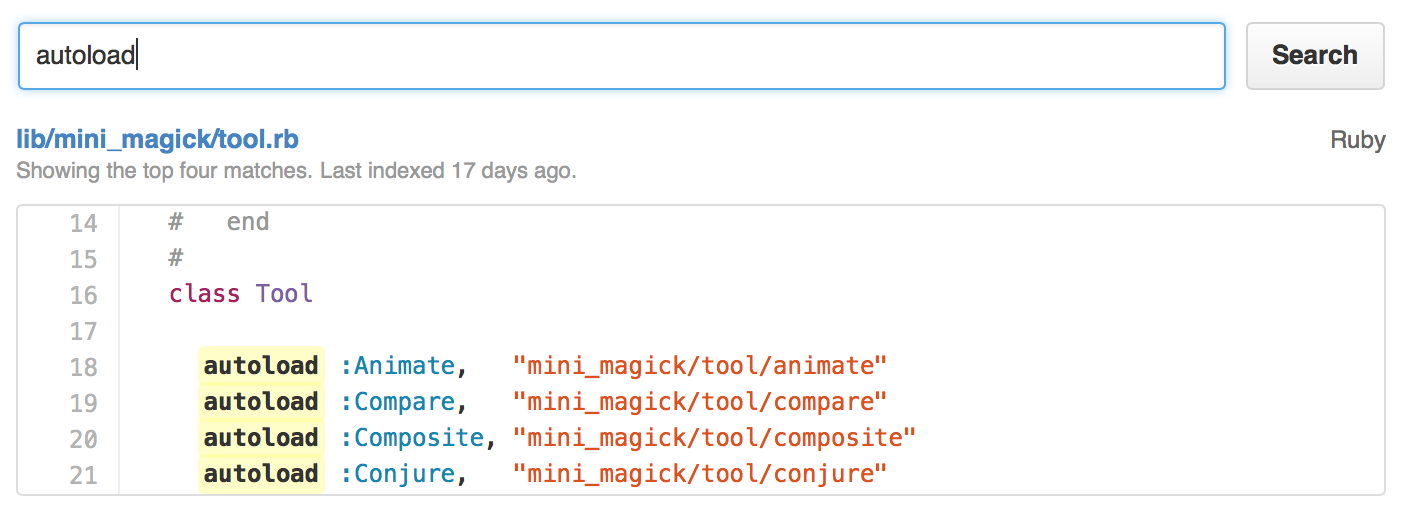
\includegraphics[width=300pt]{highlighting}
  \caption{Isticanje rezultata na \url{http://github.com}}
  \label{highlighting}
\end{figure}

\chapter{Implementacija}

U prethodnom poglavlju smo obradili sve glavne značajke koje tražilice mogu imati, a u ovom poglavlju ću napraviti uvod za praktični dio ovog rada. Praktično dio će se sastojati od implementacije pretraživanja koristeći svaku od vodećih tražilica punog teksta (koja je otvorenog koda). Najprije ću navesti i opisati svaki softver koji će se koristiti, a zatim ću opisati samu aplikaciju za pretraživanje u kojoj ću koristiti svaki softver. Cilj praktičnog dijela je primjeniti vodeće softvere na stvarnu bazu podataka, i usporediti ih na razini brzine i jednostavnosti korištenja.

\section{Softveri}

\subsection{Apache Lucene}

\textit{Apache Lucene} je programska biblioteka sa funkcionalnostima za pretraživanje punog teskta, napisana u Javi i javno distribuirana pod licencom ``Apache License 2.0''. Lucene nije potpuna aplikacija za pretraživanje, već pruža sučelje za to na nižoj razini, kroz Java API\footnote{eng. \textit{application programming interface}}.

Glavne značajke Apache Lucene uključuju:

\begin{itemize}
  \item mnogo vrsta upita (fraze, zamjenski znakovi, intervali itd),
  \item pretraživanje po poljima (e.g. naslov, autor itd),
  \item sortiranje po rangu ili proizvoljnom polju,
  \item pretraživanje po više indeksa s integriranim rezultatima,
  \item paralelno ažuriranje i pretraživanje, i
  \item ispravljanje zatipaka
\end{itemize}

Sa višeg nivoa, Lucene se koristi na sljedeći način. Prvo se inicijaliziraju dokumenti koji mogu imati jedno ili više polja. Zatim se specificira analizator dokumenata, koji će tokenizirati dokumente po poljima (ne mora se nužno koristiti analizator koji dolazi s Apache Lucene), kodek koji će kodirati i dekodirati iz invertiranog indeksa, i način kako će se indeks spremati (na disku, u memoriji itd). Nakon toga se može napraviti upit, koji prvo prolazi kroz razne analizatore (fraze, booleovi operatori itd), nakon čega se uspoređuje s indeksom, i rezultira pronađenim dokumentima.

\subsection{Apache Solr}

\textit{Apache Solr} je platforma za pretraživanje punog teksta sagrađena na Apache Lucene, napisana u Javi i javno distribuirana pod licencom ``Apache License 2.0''.

Solr se koristi tako da se pokrene kao web aplikacija, i s njom se onda komunicira preko HTTP protokola (koristeći formate JSON, XML ili CSV). Neki od glavnih URL-ova iz Solr-ovog HTTP API-a su:

\begin{description}
  \item[\texttt{POST /solr/update}] \hfill \\ Za dodavanje novih, ažuriranje i brisanje postojećih dokumenata iz indeksa.
  \item[\texttt{GET /solr/<collection>/select}] \hfill \\ Za pretraživanje indeksiranih dokumenata
\end{description}

Osim značajki koje uzima iz Apache Lucene, Solr ima i mnogo dodatnih sposobnosti:

\begin{itemize}
  \item mogućnost upravljanja bilo kojim programskim jezikom (jer se komunikacija odvija preko HTTP-a),
  \item indeksiranje mnogobrojnih formata datoteki (.pdf, .doc itd) koristeći Apache Tika,
  \item administrativno sučelje za upravljanje tražilice,
  \item geoprostorno pretraživanje,
  \item predmemoriranje (eng. \textit{caching}),
  \item nativna podrška za upravljanje valutama (npr. određivanje valute iz simbola i automatske konverzije) itd.
\end{itemize}

Neke od poznatijih organizacija koje koriste Apache Solr su AT\&T, eBay, Netflix i Disney\footnote{\url{http://lucene.apache.org/solr/}}

\subsection{Sphinx}

\textit{Sphinx} je platforma za pretraživanje punog teksta, napisana u C++u i javno distribuirana pod licencom ``GNU GPL v2.0''. Sphinx je specijalno dizajniran za dobru integraciju sa SQL bazama podataka, i da se može lako pristupiti skriptnim jezicima.

Aplikacije mogu pristupiti Sphinx-u na tri načina:

\begin{enumerate}[(a)]
  \item preko Sphinx-ove vlastite implementacije MySQL mrežnog protokola, \textit{SphinxQL}-a (ovo je preporučeni način)
  \item preko nativnog API-a za pretraživanje, \textit{SphinxAPI}
  \item kroz MySQL server sa konfiguriranim spremanjem u \textit{SphinxSE}
\end{enumerate}

Neke od glavnih značajki Sphinx-a uključuju:

\begin{itemize}
  \item nativna integracija sa svim poznatim SQL bazama (PostgreSQL, MySQL, MS SQL, Orcale itd)
  \item vrlo dobra skalabilnost i podrška za distribuiranost
  \item vrlo napredne vrste upita (npr. PARAGRAPH i SENTENCE operator i "before" operator)
  \item sve poznate elemente pretraživanja (stop-riječi, dokumenti s više polja, korjenovanje itd)
  \item vrlo napredno i potpuno konfigurabilno rangiranje na principu dodavanja faktora (blizina riječi, TF-IDF itd)
  \item sortiranje po relevantnosti ili poljima
  \item grupiranje (eng. \textit{clustering}) rezultata
  \item CLI\footnote{eng. \textit{command-line interface}} za upravljanje bazom
\end{itemize}

Neke od poznatijih organizacija koje koriste Sphinx su Tumblr i CouchSurfing\footnote{\url{http://sphinxsearch.com/info/powered/}}.

\subsection{PostgreSQL}

PostgreSQL je objektno-relacijska baza podataka, napisana u C-u i javno distribuirana pod licencom ``PostgreSQL License'' (slična BSD i MIT licenci). Iako klasične relacijske baze podataka obično nisu namijenjene vrsti pretraživanja kakvu obrađujemo u ovom radu, PostgreSQL se ističe svojim sposobnostima naprednog pretraživanja punog teksta te je validan konkurent.

Neke glavne značajke i prednosti korištenja PostgreSQL-a vezane za pretraživanje punog teksta su:

\begin{itemize}
  \item nije potreban poseban softver koji treba održavati, već se svi podaci mogu pretraživati direktno iz baze
  \item samoažurirajući indeks
  \item napredna tokenizacija (uz uobičajene karakteristike prepoznaje emailove, URL-ove, imena datoteki itd)
  \item konfigurabilno rangiranje
  \item konfigurabilni označeni rezultati
  \item dobre introspekcijske sposobnosti i testiranje
\end{itemize}

\subsection{Elasticsearch}

Elasticsearch je distribuirana platforma za pretraživanje punog teksta i analitiku u realnom vremenu, sagrađena na Apache Lucene. Napisana je u Javi i javno distribuirana pod licencom "Apache License 2.0". Elasticsearch je \textit{dokumentno-orijentirana} baza podataka, što spada u NoSQL\footnote{\url{http://en.wikipedia.org/wiki/NoSQL}} tipove baza. Slika \ref{elasticsearch} ilustrira analogiju između elemenata Elasticsearch-a i relacijskih baza.

\begin{figure}[H]
  \centering
  \begin{tabular}{lllllllll}
    RDBMS         & $\Rightarrow$ & Baze    & $\Rightarrow$ & Tablice & $\Rightarrow$ & Redovi    & $\Rightarrow$ & Stupci \\
    Elasticsearch & $\Rightarrow$ & Indeksi & $\Rightarrow$ & Tipovi  & $\Rightarrow$ & Dokumenti & $\Rightarrow$ & Polja  \\
  \end{tabular}
  \caption{Analogija između dokumentno-orijentiranih i relacijskih baza}
  \label{elasticsearch}
\end{figure}

Kao i Apache Solr, Elasticsearch također sadrži web aplikaciju s kojom se komunicira preko HTTP API-a (koristeći isključivo JSON format):

\begin{description}
  \item[\texttt{PUT /<namespace>/<type>/<id>}] \hfill \\ Za dodavanje novih, ažuriranje postojećih dokumenata u indeksu
  \item[\texttt{GET /<namespace>/<type>/<id>}] \hfill \\ Za dobivanje indeksiranih dokumenata
  \item[\texttt{GET /<namespace>/<type>/\_search}] \hfill \\ Za pretraživanje indeksiranih dokumenata
  \item[\texttt{DELETE /<namespace>/<type>/<id>}] \hfill \\ Za brisanje indeksiranog dokumenta
\end{description}

Neke od glavnih značajki Elasticsearch-a uključuju:

\begin{itemize}
  \item automatska distribuiranost
  \item jednostavan HTTP API (slijedi konvencije REST-a\footnote{\url{http://www.ics.uci.edu/~fielding/pubs/dissertation/top.htm}})
  \item nativni Java API
  \item kontrola paralelnih zahtjeva
  \item napredna introspekcija (npr. uvid zašto dokument je/nije pronađen)
  \item napredna agregacija podataka
  \item napredno i konfigurabilno rangiranje
  \item podrška za geolokacije
\end{itemize}

Neke od poznatijih organizacija koje koriste Elasticsearch su Wikipedia, The Guardian, Stack Overflow i GitHub\footnote{\cite{elastic} na \url{http://www.elasticsearch.org/guide/en/elasticsearch/guide/current/getting-started.html}}.

\section{Aplikacija}

\chapter{Rezultati}

\chapter{Zaključak}

\section{Skaliranje}

Kada gradimo aplikaciju za pretraživanje, s vremenom se broj dokumenata i broj korisnika može znatno povećati. To znači da se performanse pretraživanja mogu znatno smanjiti. Postoje razni aspekti koje možemo mjeriti da dobijemo uvid u brzinu pretraživanja:

\begin{compactitem}
  \item \textbf{Propusnost upita} – Broj upita koji sustav može obraditi u nekoj vremenskoj jedinici (npr. broj upita po sekundi).
  \item \textbf{Prosječna brzina upita} – Vrijeme koje prosječnom upitu treba da se obradi.
  \item \textbf{Statistike predmemorije} – Mnogi sistemi spremaju rezultate upita u predmemoriju (eng. \textit{cache}), i korisno je znati koliko se puta predmemorija iskoristila. Ako je predmemorija vrlo rijetko iskorištena, onda može biti brže isključiti predmemoriju.
  \item \textbf{Veličina indeksa} – Veličina indeksa je obično proporcionalna s vremenom upita.
\end{compactitem}

Prirodan način za ubrzati bilo koji računalni rad je nadogradnja hardvera. To znači da se vrijeme pretraživanja može ubrzati nadogradnjom RAM-a i procesora. Također, upotreba SSD-a (eng. \textit{solid state drive}) može znatno ubrzati vrijeme upita, iako može usporiti ažuriranje dokumenata.

Dok nadogradnja jednog računala može puno pomoći, performanse koje se mogu postići jednim računalom su svejedno ograničene. U jednom trenutku je potrebno distribuirati tražilicu na više računala (tzv \textit{skaliranje}). Tražilice punog teksta podržavaju dvije metode skaliranja:

\begin{compactenum}
  \item \textit{Replikacija} – Jedan indeks koji stane na jedno računalo se može kopirati na više računala. Na taj način se opterećenje može distribuirati po više računala. To je vrlo korisno kada je indeks relativno mali, ali je broj upita vrlo velik.
  \item \textit{Cijepanje} – Jedan indeks se može rascijepati u više dijelova (eng. \textit{shards}), i svaki dio se stavlja na zasebno računalo. Cijepanje indeksa obično internalno izvršava tražilica, ali moguće indeks rascijepati i po logičnom pravilu (npr. po govornom jeziku).
\end{compactenum}

\begin{thebibliography}{99}
  \bibitem{taming} G. S. Ingersoll, T. S. Morton, A. L. Farris, \textit{Taming Text: How to Find, Organize, and Manipulate It}, Manning Publications Co, Zagreb, 2013.
  \bibitem{lucene} \url{http://lucene.apache.org/core/4_10_3/} (siječanj, 2015)
  \bibitem{solr} \url{http://ftp.carnet.hr/misc/apache/lucene/solr/ref-guide/apache-solr-ref-guide-4.10.pdf} (siječanj, 2015)
  \bibitem{sphinx} \url{http://sphinxsearch.com/docs/latest/index.html} (siječanj, 2015)
  \bibitem{postgres} \url{http://www.postgresql.org/docs/9.4/static/index.html} (siječanj, 2015)
  \bibitem{elastic} C. Gormley, Z. Tong, dostupno na \url{http://www.elasticsearch.org/guide/en/elasticsearch/guide/current/index.html} (siječanj, 2015)
\end{thebibliography}

\pagestyle{empty}

\begin{sazetak}
\end{sazetak}

\begin{summary}
\end{summary}

\begin{cv}
\end{cv}

\end{document}
